\PassOptionsToPackage{unicode=true}{hyperref} % options for packages loaded elsewhere
\PassOptionsToPackage{hyphens}{url}
%
\documentclass[]{article}
\usepackage{lmodern}
\usepackage{amssymb,amsmath}
\usepackage{ifxetex,ifluatex}
\usepackage[margin=1in]{geometry}
\usepackage{fixltx2e} % provides \textsubscript
\ifnum 0\ifxetex 1\fi\ifluatex 1\fi=0 % if pdftex
  \usepackage[T1]{fontenc}
  \usepackage[utf8]{inputenc}
  \usepackage{textcomp} % provides euro and other symbols
\else % if luatex or xelatex
  \usepackage{unicode-math}
  \defaultfontfeatures{Ligatures=TeX,Scale=MatchLowercase}
\fi
% use upquote if available, for straight quotes in verbatim environments
\IfFileExists{upquote.sty}{\usepackage{upquote}}{}
% use microtype if available
\IfFileExists{microtype.sty}{%
\usepackage[]{microtype}
\UseMicrotypeSet[protrusion]{basicmath} % disable protrusion for tt fonts
}{}
\IfFileExists{parskip.sty}{%
\usepackage{parskip}
}{% else
\setlength{\parindent}{0pt}
\setlength{\parskip}{6pt plus 2pt minus 1pt}
}
\usepackage{hyperref}
\hypersetup{
            pdftitle={Solution of Differential Algebraic Equations with Manifold Constraints on the Latent Space of an Autoencoder},
            pdfauthor={Alejandro Francisco Queiruga},
            pdfborder={0 0 0},
            breaklinks=true}
\urlstyle{same}  % don't use monospace font for urls
\usepackage{color}
\usepackage{fancyvrb}
\newcommand{\VerbBar}{|}
\newcommand{\VERB}{\Verb[commandchars=\\\{\}]}
\DefineVerbatimEnvironment{Highlighting}{Verbatim}{commandchars=\\\{\}}
% Add ',fontsize=\small' for more characters per line
\newenvironment{Shaded}{}{}
\newcommand{\AlertTok}[1]{\textcolor[rgb]{1.00,0.00,0.00}{\textbf{#1}}}
\newcommand{\AnnotationTok}[1]{\textcolor[rgb]{0.38,0.63,0.69}{\textbf{\textit{#1}}}}
\newcommand{\AttributeTok}[1]{\textcolor[rgb]{0.49,0.56,0.16}{#1}}
\newcommand{\BaseNTok}[1]{\textcolor[rgb]{0.25,0.63,0.44}{#1}}
\newcommand{\BuiltInTok}[1]{#1}
\newcommand{\CharTok}[1]{\textcolor[rgb]{0.25,0.44,0.63}{#1}}
\newcommand{\CommentTok}[1]{\textcolor[rgb]{0.38,0.63,0.69}{\textit{#1}}}
\newcommand{\CommentVarTok}[1]{\textcolor[rgb]{0.38,0.63,0.69}{\textbf{\textit{#1}}}}
\newcommand{\ConstantTok}[1]{\textcolor[rgb]{0.53,0.00,0.00}{#1}}
\newcommand{\ControlFlowTok}[1]{\textcolor[rgb]{0.00,0.44,0.13}{\textbf{#1}}}
\newcommand{\DataTypeTok}[1]{\textcolor[rgb]{0.56,0.13,0.00}{#1}}
\newcommand{\DecValTok}[1]{\textcolor[rgb]{0.25,0.63,0.44}{#1}}
\newcommand{\DocumentationTok}[1]{\textcolor[rgb]{0.73,0.13,0.13}{\textit{#1}}}
\newcommand{\ErrorTok}[1]{\textcolor[rgb]{1.00,0.00,0.00}{\textbf{#1}}}
\newcommand{\ExtensionTok}[1]{#1}
\newcommand{\FloatTok}[1]{\textcolor[rgb]{0.25,0.63,0.44}{#1}}
\newcommand{\FunctionTok}[1]{\textcolor[rgb]{0.02,0.16,0.49}{#1}}
\newcommand{\ImportTok}[1]{#1}
\newcommand{\InformationTok}[1]{\textcolor[rgb]{0.38,0.63,0.69}{\textbf{\textit{#1}}}}
\newcommand{\KeywordTok}[1]{\textcolor[rgb]{0.00,0.44,0.13}{\textbf{#1}}}
\newcommand{\NormalTok}[1]{#1}
\newcommand{\OperatorTok}[1]{\textcolor[rgb]{0.40,0.40,0.40}{#1}}
\newcommand{\OtherTok}[1]{\textcolor[rgb]{0.00,0.44,0.13}{#1}}
\newcommand{\PreprocessorTok}[1]{\textcolor[rgb]{0.74,0.48,0.00}{#1}}
\newcommand{\RegionMarkerTok}[1]{#1}
\newcommand{\SpecialCharTok}[1]{\textcolor[rgb]{0.25,0.44,0.63}{#1}}
\newcommand{\SpecialStringTok}[1]{\textcolor[rgb]{0.73,0.40,0.53}{#1}}
\newcommand{\StringTok}[1]{\textcolor[rgb]{0.25,0.44,0.63}{#1}}
\newcommand{\VariableTok}[1]{\textcolor[rgb]{0.10,0.09,0.49}{#1}}
\newcommand{\VerbatimStringTok}[1]{\textcolor[rgb]{0.25,0.44,0.63}{#1}}
\newcommand{\WarningTok}[1]{\textcolor[rgb]{0.38,0.63,0.69}{\textbf{\textit{#1}}}}
\usepackage{graphicx,grffile}
\makeatletter
\def\maxwidth{\ifdim\Gin@nat@width>\linewidth\linewidth\else\Gin@nat@width\fi}
\def\maxheight{\ifdim\Gin@nat@height>\textheight\textheight\else\Gin@nat@height\fi}
\makeatother
% Scale images if necessary, so that they will not overflow the page
% margins by default, and it is still possible to overwrite the defaults
% using explicit options in \includegraphics[width, height, ...]{}
\setkeys{Gin}{width=\maxwidth,height=\maxheight,keepaspectratio}
\setlength{\emergencystretch}{3em}  % prevent overfull lines
\providecommand{\tightlist}{%
  \setlength{\itemsep}{0pt}\setlength{\parskip}{0pt}}
\setcounter{secnumdepth}{0}
% Redefines (sub)paragraphs to behave more like sections
\ifx\paragraph\undefined\else
\let\oldparagraph\paragraph
\renewcommand{\paragraph}[1]{\oldparagraph{#1}\mbox{}}
\fi
\ifx\subparagraph\undefined\else
\let\oldsubparagraph\subparagraph
\renewcommand{\subparagraph}[1]{\oldsubparagraph{#1}\mbox{}}
\fi

% set default figure placement to htbp
\makeatletter
\def\fps@figure{htbp}
\makeatother


\title{Solution of Differential Algebraic Equations with Manifold Constraints
on the Latent Space of an Autoencoder}
\author{Alejandro Francisco Queiruga}
\date{\today}

\begin{document}
\maketitle
\begin{abstract}
We train an autoencoder to determine the lower-dimensional
representation of the EOS surface using modern deep learning techniques
without using any phase labels. The decoder end of the model is then
plugged back into the balance laws, eliminating the constraint equation.
\end{abstract}

\begin{center}\rule{0.5\linewidth}{\linethickness}\end{center}

\hypertarget{header-n3216}{%
\section{Introduction}\label{header-n3216}}

Representing complex physical systems with multiple speicies, phases,
chemical reactions, and heterogenous scale effects poses an
intractability problem to modeling. How do we analyze complex
experimental data and \emph{ab initio} simulations and derive new
macroscale relations to describe the systems? How do we then implement
these relations in the rest of our analyses and production-scale
computer simulations?

Accurately simulating multispecies reaction and transport with
undergoing phase transitions is a critical aspect to a variety of
problems.
Motivations for this work are subsurface energy systems such as shale
and oceanic natural gas reservoirs in shales or engineered geothermal
systems.

A single material with multiple phase transitions
is a challenge in of itself, and the descriptions become combinatorially
more complex as species and phases are added. This results in
combinatorially more human labor and combinatorially more code which
tends to involve complex branching logic. The descriptions then pose
numerical challenges when incorporated into macroscale simulations due
to obstacles such as discrete phase state machines and primary variable
switching.

The system of equations we are looking at are, for only two components,
\begin{align}
  \partial_t \rho_{H_2O} =& \nabla \cdot flux_{H_2O} + s \\
  \partial_t \rho_{CO_2} =& \nabla \cdot flux_{CO_2} + s \\
  \partial_t e& = \nabla \cdot flux_{heat} + s
\end{align}
More species add more rows, and applicaitons also involve continuum
mechanics and chemical reactions! The interplay of deformations,
reactions, and phase transitions makes the equations extremely difficult
to solve. \cite{my millstone paper}

This work only considers the "single beaker" problem; the flow
and transport aspects have similar challenges. (The next stage of this
work will "connect the beakers".)

In section 2, we will cast the above equation into a basic form for a
differential algebraic equation,
\begin{align}
  z( u, \partial_t u) &= 0 \\
  c(u) & = 0
\end{align}
We will introduce a new way of thinking about constraints as sets of
solutions or observations of possible $u$:
\begin{equation}
c(u)=0 \leftrightarrow \left\{ u | c(u)=0 \;\text{or}\; u\; \text{observed} \right\}
\end{equation}
We will use this set of possible values viewpoint to train an
autoencoder on the set of $u$ for a latent space parameterized by $q$:
\begin{equation}
u = D(q), \; q=E(u) \;\forall u \in U
\end{equation}
which satisifies
\begin{equation}
  D(q)\in U \forall q.
\end{equation}
We can then write the original equation by
\begin{equation}
z(q,\partial_t q)=0
\end{equation}





Part of the new modern software engineering framework involves replacing
human-written code with computer-written code. We are applying this
mindset from industry problems in the Artificial
Intelligence space into scientific computing.

The actual meaning of the parameterization is not important, so long as
it can be effectively solved and then \emph{decoded} back to the
physically meaningful quantities.

We redescribe our problem as a differential algebraic equation
with a constraint: the balances of mass and energy are constrained by
the EOS. Because the EOS was originally derived from data, a data-driven
approach lends itself in which the EOS is a set of points in
temperature-pressure-density-enthalpy space. (In the multicomponent
cases there are more dimensions.)

We demonstrate this approach to solving constrained differential
equations on the pendulum, before demonstrating two EOSes of water: one
with just liquid-gas phases, and one with liquid-gas-ice-supercritical
regimes. The notion of phases does not appear in this multiphase
simulation. We show a model architecture that is able to learn phase
labels in the unsupervised autoencoder training process, such
human-scientist interpretable results are obtained from the machine
learning process. We compare this and other model architectures,
including common deep neural networks, based on autoencoder error and
simulation success metrics. We stress that the presented approach is
only utilizing machine learning on material relations derived from
empirical data: the simulation is indeed solving physical balance laws.

Our proposed approach is to build upon modern machine learning
techniques to aid in equation discovery. An autoencoder is trained on
the original material dataset to learn a lower-dimensional
representation of the underlying manifold. The model is designed to be
directly incorporated into a macroscale simulation of physical balance
laws, where now the traditional partial differential equations are being
solved on the learned latent space. This provides a more robust
numerical algorithm, while putting the onus of programming part of the
simulation itself onto the computer: tens of thousands of lines of human
written code consisting of empirical fits and branching logic are
replaced by code generated by the learned model. The methodology will
first be demonstrated on datasets based on thermodynamic intensive
variables, which are already challenging to analyze, before being
extended to richer datasets such as experimental images or molecular
dynamics. We stress that the proposed approach is only utilizing machine
learning on material data: the simulation is indeed solving physical
balance laws. Through deep learning approaches combined with
domain-specific goals, we can learn feature sets that are both
interpretable and directly apply to analyzing larger systems.



This work proposes a new methodology that steps away from the
traditional approaches. 
In this approach, we directly \emph{look for solvable representations}
instead of representations that carry human intuition. We value
simulation runtime and robustness. Further, we must remember the value
of the human effort involved: beyond improving computational aspects,
we are fully automating part of the human involvement in programming
the simulator.

In section 2, the balance of mass and energy will be described for a
single multiphase material. We will discuss the current state of the
art algorithm for deriving relationships for multiphase materials, and
then the primary-variable switching algorithm that is used in
state-of-the art solvers. The equation will then be recast as a
constraint problem in th above form.
In section 3, we will demonstrate applying the autoencoder learning
methodology to solve the pendulum,
which can be considered the archetypical constraint problem.
In section 4, the autoencoder methodology wil lbe applied to the
equation of state of water. In section 5, the new simulation process
will be described, wherein the learned decoders are placed into the
balance laws, forming newly discovered equations on learned
representations. The software implementation of the training and
simulation programs are detailed in section 6. The new simulation
framework on sets of learned representations is evaluated on
multiple datasets of varying extents of water with a
hyperparameter search on a suite of test problems to prouce the discussion of section 7, as
well as a systematic automated testing procedure of a
machine-dominated programming methodology.
Active research and software development directions are
concluded in the final section.

The notebooks and software implementations are released open source to
accompany this work. They can be found at the github repository
located at: \href{https://github.com/afqueiruga/latentsim}
Certain components are factored into submodule repositories which are
each released under the LGPL at seperate repositories referenced in
the implementation details.

\hypertarget{header-n3234}{%
\section{Multiphase Equations of State}\label{header-n3234}}

For this preliminary work, we consider only a single-beaker problem
without flow. Let \(\rho\) be the material density, \(T\) be the
temperature, \(p\) be the material pressure, \(h\) be the material
enthalpy, and \(u\) be the internal energy. There are two equations for
balance of mass and energy.

\begin{align}
\partial_t \rho & = \mathbf{k}_p(p_\infty - p) + r\\
\partial_t \rho u & = \mathbf{k}_T(T_\infty-T) + s
\end{align}

The beaker is exposed to a reservoir with \(p_\infty\) and \(T_\infty\)
via a mixed boundary condition straw with transport and conduction
coefficients \(\mathbf{k}_p\), \(\mathbf{k}_T\). Mass and heating
sources and sinks are the terms \(r\) and \(s\).\footnote{We express the
  material by enthalpy instead of internal energy; they are related by
  the relation \(\rho u = \rho h - p\). Future work may work directly
  with internal energy.}

The typical methodology is to use the empirical relations for density
and enthalpy \(h\) as a function of pressure and temperature and solve
the DAE for \(p\) and \(T\) implicitly:

\begin{align}
\text{Solve for}\, p(t)\, \text{and}\, T(t)\, \text{such that:}\\
\partial_t \rho(p,T) & = \nabla \cdot \mathbf{k}\nabla p + r\\
\partial_t \rho u(p,T) & = \nabla \cdot \mathbf{k'}\nabla T + s
\end{align}

The complicatation is that the functions \(\rho(p,T)\) and \(u(p,T)\)
are not well defined functions due to the presence of phase changes that
yield sharp discontinuities in \(p,T\), as shown in Figure 1 for
water.

We also consider the phase equilibria; at a larger scale it is possible
for a control volume to be a mixture of two phase coexisting, such as
boiling with some mixture saturation \(S_{gas}=1-S_{liq}\).
(For a very fine scale simulation, bubbles would be explicitly modeled.)
The material can exist on this section of the surface as a mixture of
the two phases.

\[\rho = X_{H_2O}\left(S_{gas} \rho_{gas} + S_{liq} \rho_{liq} + S_{ice} \rho_{ice} + S_{crit} \rho_{crit} \right)\]



One possible definition of phase boundaries:

\begin{quote}
Phase transitions occur when the thermodynamic free energy of a system
is non-analytic for some choice of thermodynamic variables (cf. phases).

https://en.wikipedia.org/wiki/Phase\_transition
\end{quote}

\begin{figure}
\centering
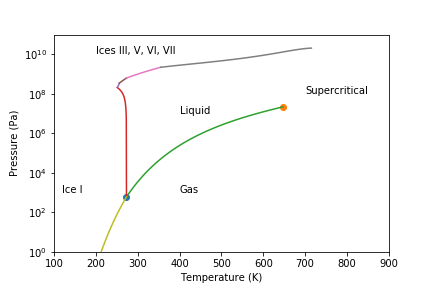
\includegraphics{/Users/afq/Documents/Dropbox/ML/primaryautoencoder/figures/phase_diagram.png}
\caption{Phase boundaries for water }
\end{figure}

\begin{figure}
\centering
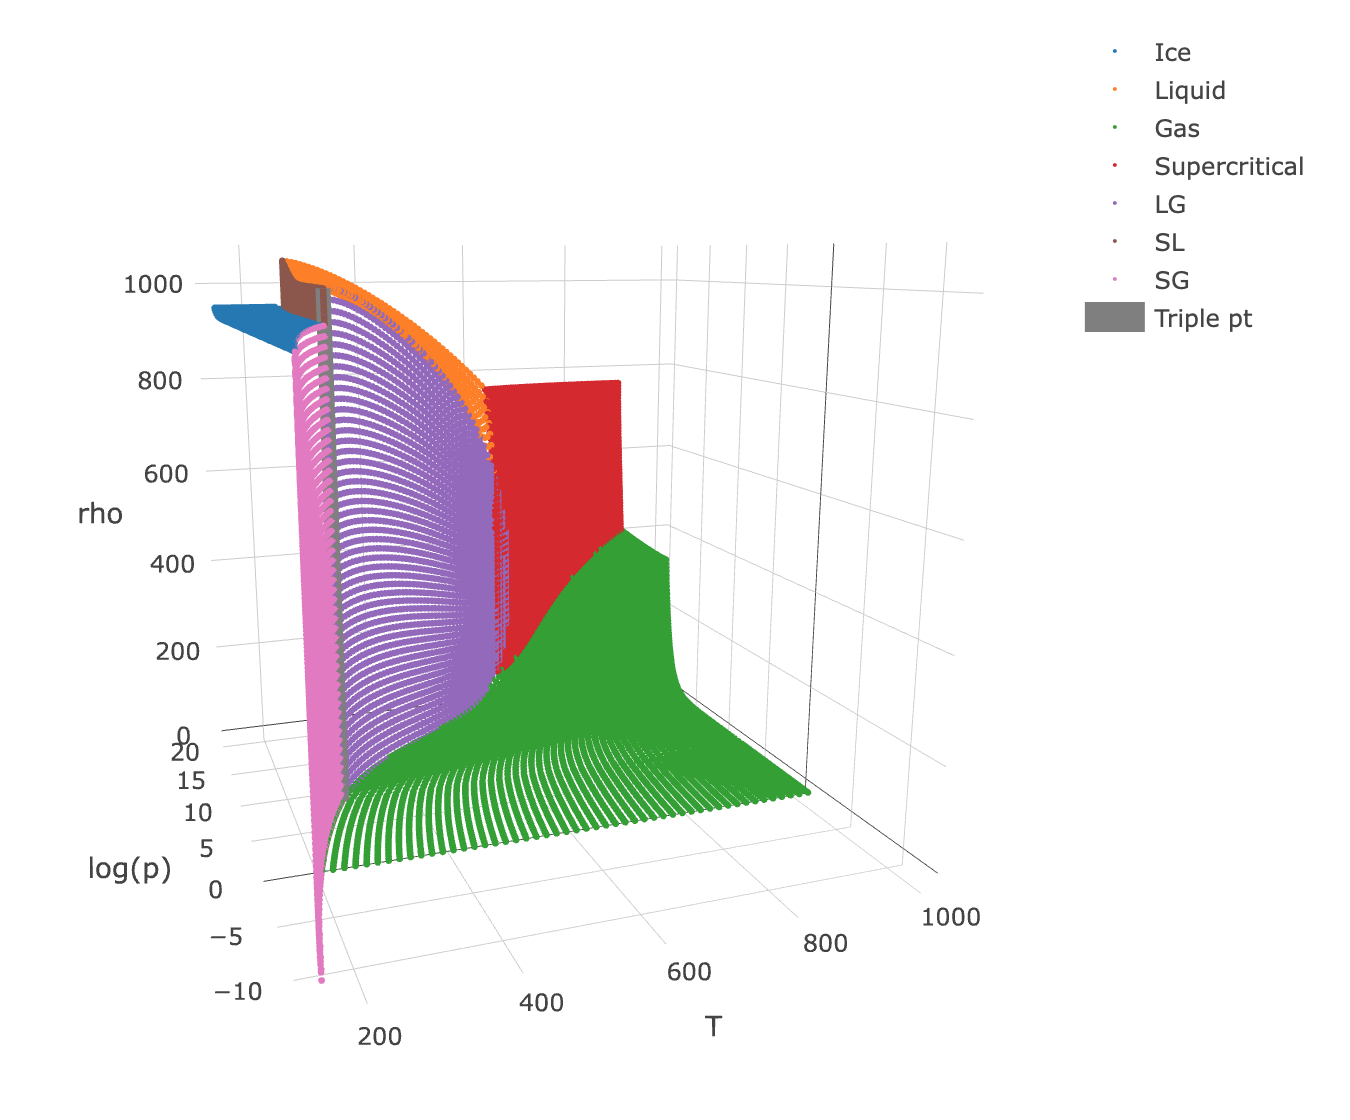
\includegraphics{/Users/afq/Documents/Dropbox/ML/primaryautoencoder/figures/water_eos.png}
\caption{\label{fig:pTrho} The $\log{p}$, $T$, $\rho$ equation of
  state surface for water. This plot spans four phases, three
  equilibria, and the triple point, which are each given their own color.
  There is a fourth dimension to the surface of enthalpy $h$ that exhibits
  similar discontinuities; the $\log{p}$, $T$, $h$ surface is plotted
  in the Appendix.}
\end{figure}

There are even more known phases of crystal ice which for water
For water, the supercritical phase and exotic ices only occur in
laboratory conditions or naturally near the
crust \cite{}. For other materials these exotic phases can be
applicable. For example, in geoengineered systems using $CO_2$
such as geothermal plants are carbon sequestration facilities, the
working fluid is usually in the supercritical regime at depth.

\hypertarget{header-n3253}{%
\subsection{State Machine logic}\label{header-n3253}}

Formulate balance equations as

\[R(X ; phase) = 0\]

Solve the differentiable part:
\[\frac{\partial R}{\partial X}\Delta X^{k+1/2} = -R(X^k ; phase^k)\]
and iterate on the nondifferential part:
\[phase^{k+1},X^{k+1} = statemachine(X^{k+1/2} ; phase^k)\]
The phase switching logic has the form of a switch case:

\begin{Shaded}
\begin{Highlighting}[]
\ControlFlowTok{switch}\NormalTok{ phase_old:}
  \ControlFlowTok{case}\NormalTok{ gas:}
    \ControlFlowTok{if}\NormalTok{ p,T crossing boundary:}
\NormalTok{      phase_new = liquid_gas}
  \ControlFlowTok{case}\NormalTok{ liquid:}
    \ControlFlowTok{if}\NormalTok{ p,T crossing boundary:}
\NormalTok{      phase_new = liquid_gas}
  \ControlFlowTok{case}\NormalTok{ liquid_gas:}
    \ControlFlowTok{if}\NormalTok{ S_gas >= }\DecValTok{1}\NormalTok{:}
\NormalTok{      phase_new = gas}
    \ControlFlowTok{if}\NormalTok{ S_liquid >= }\DecValTok{1}\NormalTok{:}
\NormalTok{      phase_new = gas}
\end{Highlighting}
\end{Shaded}

\hypertarget{header-n3262}{%
\subsection{A constrained Differential Algebraic
Equation}\label{header-n3262}}

We argue that the relations that are used are not the \emph{ground
truth} in of themselves. Beyond ideal gases and simple linear fluids,
the functions \(\rho(p,T)\) or \(p(\rho,T)\) are simply complicated fits
that were derived in an ad-hoc piecewise fashion from experimental data.
This is not a bad thing---it is the fundamental nature of the problem.
When we look at the corpus of literature on a material as water, what we
actually have is a decision branch to multiple different complicated
fits for each material branch.

We instead replace our problem with two balance laws and one unknown
constraint:

\begin{align}
\text{Solve for}\, \rho(t), \, h(t), \, p(t),\, \text{and}\, T(t)\, \text{satisfying:}\\
\partial_t \rho & = \nabla \cdot \mathbf{k}\nabla p + r\\
\partial_t \rho h - p & = \nabla \cdot \mathbf{k'}\nabla T + s\\
\text{such that they lie on the material EOS,}\\
EOS(\rho,h,p,T) & = 0
\end{align}

The \emph{ground truth} is the experimental data in the first place; the
branching curve fit is only one realization of representing the data. We
have demonstrated that it is not possible to represent any two of these
in terms of the other two; and even if so, it is not necessarily a good
and robust fit. What if we search for a new fit?

\hypertarget{header-n3267}{%
\section{The Pendulum}\label{header-n3267}}

An archetypical constraint problem the pendulum. Posed as dynamics
problem with a Lagrange-multipler-esque centripetal force, it
has three unknowns wtih two second-order equations and a constraint,

\begin{align}
\text{Solve for}\, x(t), \, y(t), \, f(t) \, \text{satisfying:} \\
m \ddot{x} & = f x/\sqrt{x^2+y^2} \\
m \ddot{y} & = f y/\sqrt{x^2+y^2} - m g \\
x^2 + y^2 & = R^2
\end{align}


Note that we are considering the nonlinear pendulum.

There are many ways to solve this cannonical equation: Lagrange
multipliers (\(f(t)\) is the multiplier in the way we have written it
above), penalties, change of variables, etc. The change of variables
method exploits the Lagrangian mechanics formulation, where we state
the Lagrangian,
\begin{equation}
L = \frac{1}{2}m\left(\dot{x}^2 + \dot{y}^2\right) - m g y
\end{equation}
with the constraint that \(x\) and \(y\) lie on the path.
We can introduce a new variable \(\theta\) that parameterizes
\(x=R\cos\theta\) and \(y=R\sin\theta\) and rederive the equations of
motion with the familiar,
\begin{align}
\text{Solve for}\, \theta(t) \ \text{satisfying:} \\
\frac{\mathrm{d}}{\mathrm{d}t} \frac{\partial L}{\partial
  \dot{\theta}} =
  \frac{\partial L}{\partial \theta}
\end{align}
In this example, this lets us collapse the problem into a
single-component second-roder differential equation.

In our methodology, we do not have an explicit equation for the
constraint, but a dataset of $X$ of $(x,y)$ pairs that are on the manifold. For
our proof-of-concept test, we manufacture this data for the circular
pendulum to verify against the analytical solution:
\begin{equation}
X = \left\{ (R\cos\theta_i, R\sin\theta_i)\; | \;\theta_i \in [-5\pi/4,\pi/4] \right\}
\end{equation}
We also try a ``goofier'' looking curve with no known closed form
solution to exercise the methodology,

(For the equation of state problem, this is analogous to the dataset
of $p,T,\rho,h$ 4-tuples that make the plot in Figure \ref{fig:pTrho}.)

The manifold for this simple problem is smooth, so two nested
polynomials forms the autoencoder:
\[\left\{\begin{array}{c} x\\y\end{array}\right\}
\rightarrow W_{enc} x^n \rightarrow q \rightarrow W_{dec} x^n \rightarrow 
\left\{\begin{array}{c} x\\y\end{array}\right\}\]

(We explicitly write the bias \(+b\); it is equivalent to including
\(x^0=1\) in the polynomial set.)
The equations
of motion given some parameter space that satisfies the constraint is

\begin{equation}
\frac{\mathrm{d}q}{\mathrm{d}t}\frac{\partial L}{\partial \dot{q}} = \frac{\partial L}{\partial q}.
\end{equation}

We'll use the autoencoder to generate the parameterization of \(x(q)\)
and \(y(q)\). By the chain rule, the velocities are related to the
feature space by

\begin{equation}
\dot{x} = \frac{\mathrm{d}x(q)}{\mathrm{d}t} = \frac{\partial x}{\partial q}\frac{\mathrm{d}q}{\mathrm{d}t}
\end{equation}

and similarly for the \(y\) direction.

Taking the partial derivatives with respect to the feature variable and
its rate, the components to the equation of motion are

\begin{equation}
\frac{\partial L}{\partial q} = m g \frac{\partial y}{\partial q}
\end{equation}

When we want to solve the dynamics, we can treat the autoencoder the
same as \(x(\theta)\), plugging in

\[L(x(q),v(q,\dot{q}))\]

and build the DAE we know from physics:

\[\frac{\mathrm{d}}{\mathrm{d}t}\frac{\partial L}{\partial \dot{q}} = \frac{\partial L}{\partial q}\]

where we get the velocity with the chain rule:

\[v = \frac{\partial x}{\partial q} \dot{q}\]

Then plug it into a Runge Kutta (trapezoidal) to solve with Newton's
method:

\[\frac{\partial L}{\partial \dot{q}}_i - \Delta t \frac{\partial L}{\partial q}_i = \frac{\partial L}{\partial \dot{q}}_0 + \Delta t \frac{\partial L}{\partial q}_0\]

\begin{figure}
\centering
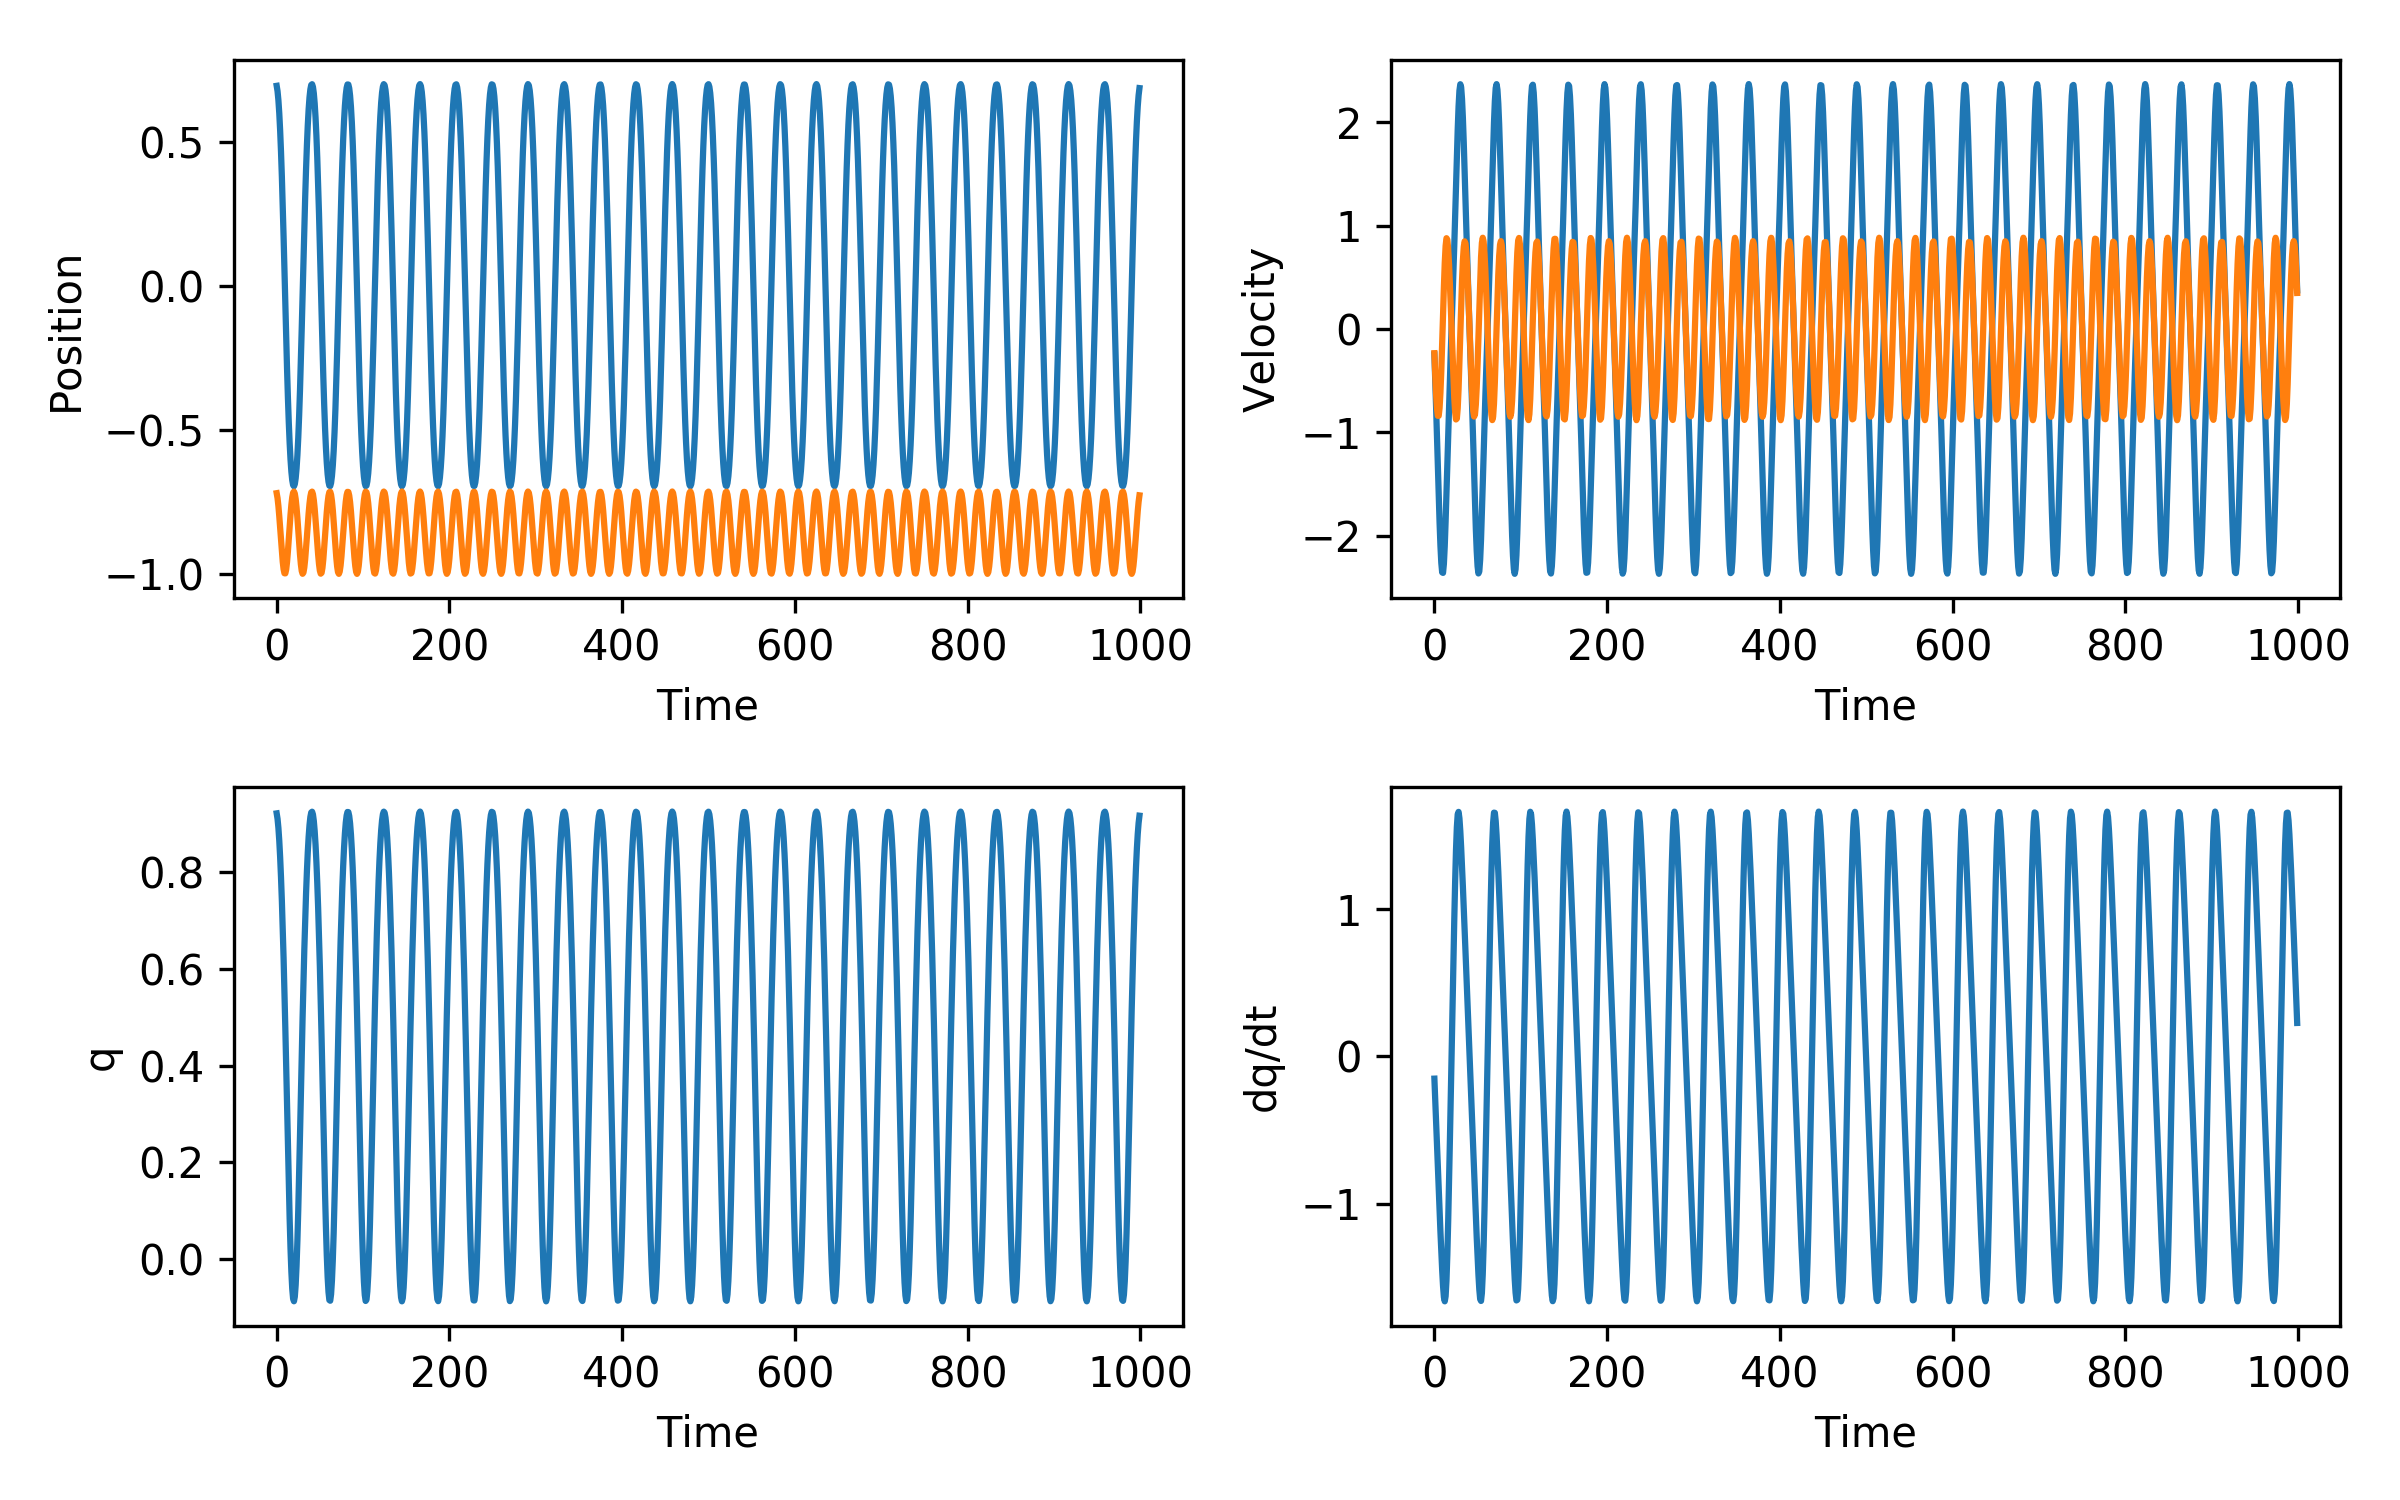
\includegraphics{/Users/afq/Documents/Dropbox/ML/primaryautoencoder/figures/pendulum_q.png}
\caption{}
\end{figure}

\hypertarget{header-n3294}{%
\section{Representation Learning for
Reparameterization}\label{header-n3294}}

The central idea of this work is to obtain two new variables solve for
those directly,

\begin{align}
\text{Solve for}\, u(t)\, \text{and}\, v(t)\, \text{such that:}\\
\partial_t \rho(u,v) & = \nabla \cdot \mathbf{k} \nabla p(u,v) + r \\
\partial_t \rho e(u,v) & = \nabla \cdot \mathbf{k'}\nabla T(u,v) + s
\end{align}

where \(u\) and \(v\) have no physical meaning other than simply being a
parameterization of the equation of state constraint. We want to select
\(u\) and \(v\) to require no auxilary phase index to define the system
and no additional logic in the code. The sharp kinks and possible
discontinuities can be a part of the functions
\(\rho(u,v), p(u,v), e(u,v)\) and \(T(u,v)\).

Can we automatically discover this parameterization? (For a such a
simple equation, we do not think the proposed methodology will be
better, but the pendulum will instead be our \emph{unit test}.) Our
proposed method is motivated by the problems of multiphase reaction and
transport, where the underlying constraints are the ill-behaved material
properties which are difficult to describe. We change our perspective on
these problems in the next section.

\hypertarget{header-n3299}{%
\subsection{Latent Space}\label{header-n3299}}

Instead of the painstaking work of parameterizing phase boundaries and
determining curve fits by hand, we rephrase the problem of representing
the equation of state by learning and autoencoder. We have an encoding
phase, \(E(\rho,p,e,T; a)\) and a decoding phase, \(D(u,v; b)\) that
forms an identity function with a compressed subspace:

\begin{equation}
\left\{ \rho, p, e, T \right\} \rightarrow  E \rightarrow \left\{ u,v \right\} \rightarrow D \rightarrow \left\{ \rho, p, e, T \right\}
\end{equation}

The autoencoder is solved for by optimizing its parameters using the
goal

\begin{equation}
\min_a \sum_x \left( x - D(E(x;a);a) \right)^2
\end{equation}

Note that we are not yet considering constraints \(c\) with partial
differential equation components in space. These types of material
equations of states are only enforced pointwise. The time components of
the equations can contain spatial derivatives; i.e. this method fits
easily inside a finite volume simulation with little change.

\hypertarget{header-n3305}{%
\subsection{Training}\label{header-n3305}}

We use a Euclidean norm loss function with a contractive penalty:

\[L(x)=\left\|x-D(E(x))\right\|^2_2+\lambda\left\|\frac{\partial E}{\partial x}\right\|_F^2\]

The gradient on the encoder is a \(4\times2\) matrix in our case, and
\(\|\|_F\) denotes the Frobenius norm. The contractive penalty
\(\lambda\) smooths out and evenly distributes the mapping to \(q\).

The variational autoencoder is a little more complicated to implement,
and we do not necessarily want to match a Gaussian interior. Because we
generated our datasets artificially (both in this manufactured setting
and in an actual laboratory setting), the dataset does not reflect draws
from a distribution, so the KL divergence against a gaussian is not
quite applicable.

We note that penalizing the decoder would smooth out the sharp kinks at
phase boundaries.

The dataset is split into a standard $2/3-1/6-1/6$ division into
training-testing-validation groups. We note that we can always
manufacture more datapoints. We train by alternating phases. The first
step is minibatched stochastic descent on the entire deep network, assembling the losses on minibatches of the data, $X_{mini}$,
\begin{equation}
  L(X_{mini}) = \sum_{x\in X_{mini}} L(x)
  \end{equation}
to perform the out-of-the-box ADAM optimizer on all of the
parameters in the networks. (The box is
TensorFlow.) After a few epochs of this,
the training algorithm alternates to a few steps step of linear regression on the last layer of the network,
denoted by \(W^{dec}\), which directly controls the magnitudes of the values.
(The bias $b^{dec}$ is included in $W^{dec}$.) The linear
system that needs to be solved is easily generated by assembling the
gradient and Hessian of the total loss function,
\begin{align}
 \mathbf{G}\left(X_{train}\right) &= \sum_{x\in X_{train}}\frac{\partial L}{\partial W^{dec}} \\
\mathbf{H}\left(X_{train}\right) &= \sum_{x\in X_{train}}\frac{\partial^2 L}{\partial (W^{dec})^2}
\end{align}
and solving the linear system for an update to the last parameters.

\[[\mathbf{H}] \Delta W^{dec} = -\{\mathbf{G}\}\]

To form the hessian and gradient for this step, we sum over all of the
training data. (The contractive penalty term drops out because it does
not depend on \(W^{dec}\).)

In future work, we would want to continue appending new \(q\)s in a
systemic way to derive, e.g., an \(H_2O + NaCl\) equation of state with
3 degrees of freedom, bootstraping from the pre-trained \(H_2O\)
architecture with 2 degrees of freedom.

\hypertarget{header-n3312}{%
\subsection{Encoder Initializations}\label{header-n3312}}

The properties \(p,T\) are the usual prefered choice for primary
variables, but as discussed above, the equations of state are not
analytic for any choice. (Indeed, this idea first spawned when the
author was thinking about systematically rewriting equations in
\(\rho,h\).) Ideally, this system would be fully automated, but due to
the nonlinearilty of the autoencoder problem there are many "bad"
options the trainer can fall into. Multiple starts are possibly needed
to get a good solution when starting from purely randomized newtork
parameters. Global optimization is truly a necessity when trying to
optimize networks with so few parameters. We incorporate a little bit of
human intuition and preference by trying three options to start off the
autoencoder: 1) fully random, 2) \(p,T\) prefered, 3) \(\rho,h\)
prefered. This is implemented by added a bias to the initialization of
the encoder coefficients, e.g. for \(p,T\),
\begin{equation}
 W^{init}_{enc} = \left[\begin{array}{ccccc}
1 & 0 & 0 & 0 & ... \\
0 & 1 & 0 & 0 & ...
                        \end{array}\right]+[\sigma]
\end{equation}
where \([\sigma]\) is the random initialization and \(…\) denotes
padding the coefficients to the nonlinear terms by 0s. Recall that the
values for \(s\) have already been rescaled to be around 0 with a range
of 1. The random initialization part is decided by
\(\sigma \sim \mathcal{N}(0,0.1)\) .

\hypertarget{header-n3317}{%
\subsection{Unsupervised Phase Classification}\label{header-n3317}}

\begin{figure}
\centering
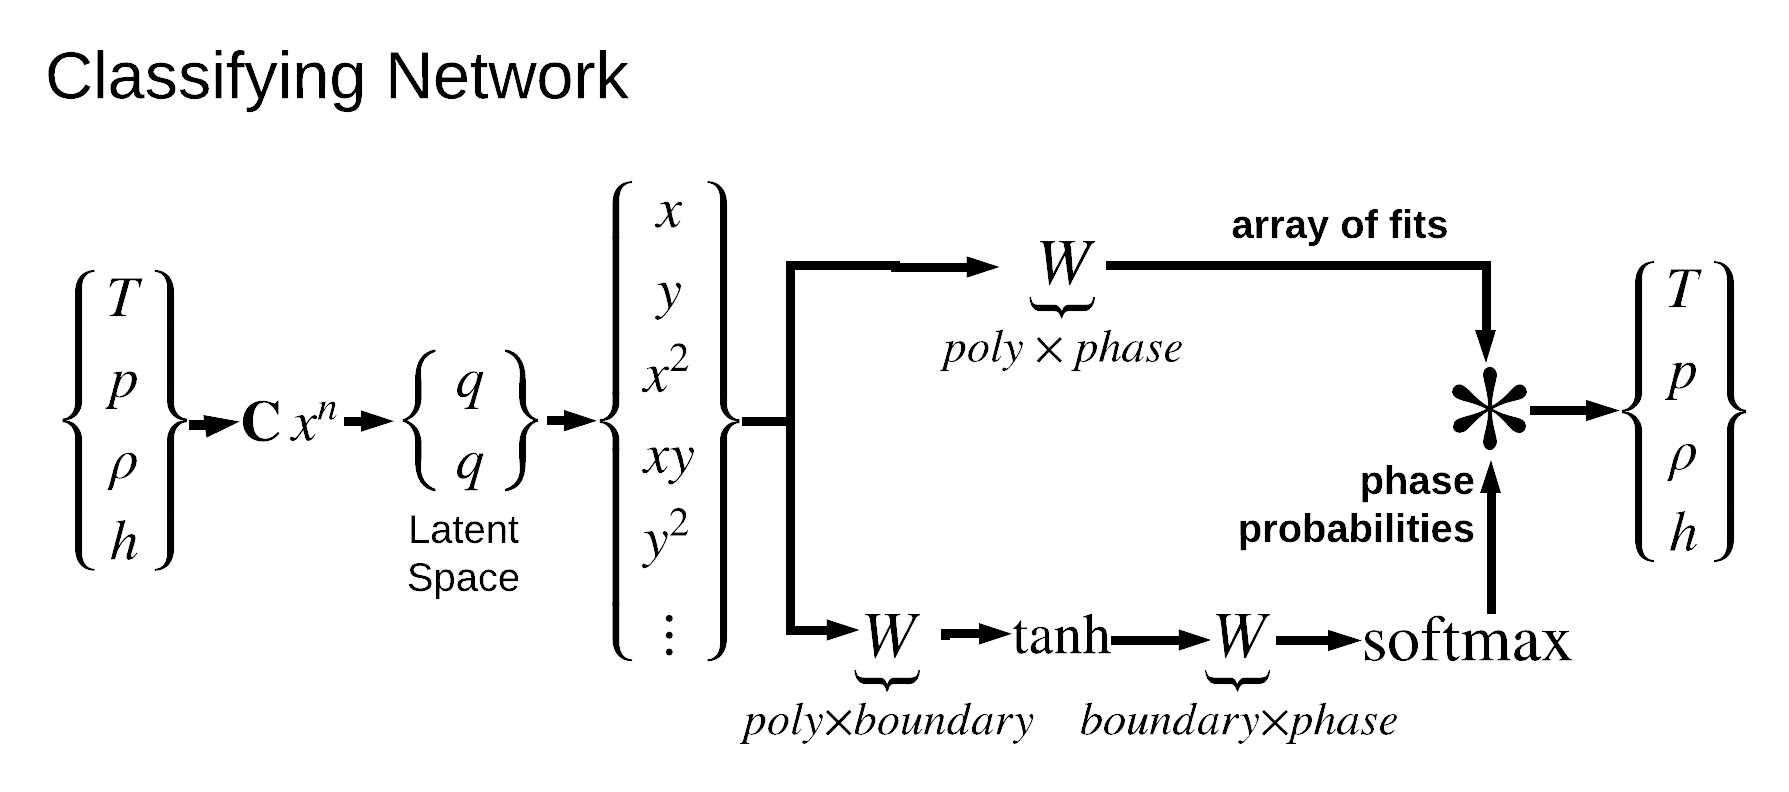
\includegraphics{/Users/afq/Documents/Dropbox/ML/primaryautoencoder/slides/classifier_network.png}
\caption{The architecture of the classifier network designed for
  unsupervised labeling of phases.}
\end{figure}

\hypertarget{header-n3321}{%
\section{Simulation}\label{header-n3321}}

Solve for \(q_1(t)\) and \(q_2(t)\) such that:

\begin{align}
\partial_t \rho(q_1,q_2) & = \nabla \cdot \mathbf{k} \nabla p(q_1,q_2) + r \\
\partial_t \rho h(q_1,q_2)-p & = \nabla \cdot \mathbf{k'}\nabla T(q_1,q_2) + s
\end{align}

where \(\rho(q_1,q_2)\) etc. are the back of an autoencoder:

\begin{equation}
\left\{ \begin{array}{c}
T\\ p\\ \rho\\ h
\end{array}\right\} \rightarrow  E \rightarrow 
\left\{ \begin{array}{c} q_1\\q_2 \end{array} \right\}\rightarrow D \rightarrow 
\left\{ \begin{array}{c}
T\\ p\\ \rho\\ h
\end{array}\right\}
\end{equation}

Using the autoencoder to automatically remove the local constraint:

\begin{equation}
eos(D(q_1,q_2)) = 0 \, \forall \,q_1,q_2
\end{equation}

\textbf{Only training the material representation, not the balance
laws.}

First, we had a constrained DAE:

\begin{align}
\frac{\mathrm{d}}{\mathrm{d}t} m(T,p,\rho,h) &= r(T,p,\rho,h)\\
eos(T,p,\rho,h) &= 0
\end{align}

with no good representation of \(eos\) everywhere.

The autoencoder parameterizes the constraint :

\begin{equation}
\frac{\mathrm{d}}{\mathrm{d}t} m(D(q)) = r(D(q))
\end{equation}

We can parameterize this equation with any time stepping scheme, .e.g. a
Runge-Kutta scheme. For subsurface flow, backward Euler is popular due
to its simplicity and L-stability, which we follow since the topic of
this paper is not exploring new time stepping schemes. This yields the
discretizated algebraic equation for \(q_i\) at \(t+\Delta t\) given the
value \(q^0\) at \(t\),

\begin{equation}
0 = R(q^i) = m(q^{i}) - m(q^{0}) - \Delta t \, r(q^i)
\end{equation}

where we have called the quation \(R(q)\). By design \(R(q)\) is smooth
enough to solve with Newton's method without any statemachine logic:

\begin{equation}
\frac{\partial R}{\partial q} \Delta q^{k+1} = R(q^k)
\end{equation}
This equation is deceptively simple: the function \(R(q)\) has complex logic encoded in it; if-then
statements appear if the model used activations such as rectifiers.
However, the complex material behavior which traditionally requires
the vast majority of programming was implemented automatically by the
models; implementing equations XX, XX, and XX require only a few lines
of human-written code. 

\hypertarget{header-n3339}{%
\subsection{Initialization}\label{header-n3339}}

There is a caveat with representing the degrees of freedom of the system
on a learned space: the user does not know the meaning of \(q\) as an
input. Further, the values of \(q\) vary from network to network and
depend on the parameterization. The user needs to be able to specify the
"real" physical quantities.

Since the original manifold is 2D, the user only needs to specify two
initial values. In a multiphase solver such as TOUGH, the state needs
to be specified with the two primary variables plus the state tag: 
\begin{verbatim}
9e5 20 Aqu
0.5 20 AqG
\end{verbatim}
Note that the first primary variable means pressure in the first line
for a pure-liquid state,
but saturation in the second line for the liquid-gas equilibrium.
This makes sense inuitively, as this is how humans are taught, but
still leads to bugs and occasionally requires looking up values in
textbooks or the manual. (Is it $S_{gas}$ or $S_{aqu}$ on the second
line?) A fully fledged solver needs to check the user specified
initial conditions for erroneous inputs.

For LatentSim, the input system is not yet as robust as a
fully-fledged user-facing simulator, but the inputs are specified in
the $T p \rho h$ space instead of the $q$ space.
The user (or test problem) specifies any two of the four values in a
dictionary format,
\begin{verbatim}
p=9e5 T=20
rho=500 T=20
\end{verbatim}
Then, the simulator must determine $q(t=0)$ from these two
values. This sets up a system of two equations.

Note that the encoder only necessarily works when all four values are
correct. Thus, it is necessary to actually solve the nonlinear problem
on the decoder:
\[D(q^0)_i = s^0_i \quad \text{for specified}\; i\]
This equation has two rows indexing into the four state variables;
e.g. only the rows associated with $p$ and $T$ are solved if those are
specified, which is usually the case. The above equation is solved
with Newton's method. The two corresponding rows are cut out of
the tangent matrix to $D$,
\[K_{ij} = \frac{\partial D_i}{\partial q_j}  \quad \text{for specified}\; i, \text{for}\;j=1,2\]
and the following system of equations is solved for an update to $q$,
\[K\Delta q = s^0_i-D(q)_i\]
Updating $q$ is repeated until convergence.

The initial condition problem is not gaurunteed to converge, however,
and often does not.
For example, if the initial guess was in the liquid phase and the target point
in the EOS space is in a solid, the iteration will fail.
To address this issue, we perform multiple starts with an initial condition in each
phase and equilibrium, discard points that diverge, and then pick the
\(q\) that is closest to the two specified components. The multiple
start points are specified at EOS development time to form a set of
values that represent middle points for each phase,
\begin{equation}
\left\{s_{guess}\right\} = \left\{ \left(\begin{array}{c}
\bar{T}_{gas}\\
\bar{p}_{gas}\\
\bar{\rho}_{gas}\\
\bar{h}_{gas}
\end{array}\right),\left(\begin{array}{c}
\bar{T}_{liq}\\
\bar{p}_{liq}\\
\bar{\rho}_{liq}\\
\bar{h}_{liq}
\end{array}\right),\left(\begin{array}{c}
\bar{T}_{ice}\\
\bar{p}_{ice}\\
\bar{\rho}_{ice}\\
\bar{h}_{ice}
\end{array}\right)... \right\}
  \end{equation}
The multistart method could be specified without any prior knowledge
with random points, but this is a sufficiently robust method for
now. Each of the possible guess points is used to fill in the two
unspecified values as guesses and then passed into the encoder.
E.g. if $p$ and $T$ were specified, each possible $\bar{\rho}$ and
$\bar{h}$ combination from the above sets are filled in to provide
multiple guesses for $q$,
\begin{equation}
s^0 = \left(\begin{array}{c}
T^*(0)\\
p^*(0)\\
\bar{\rho}_{guess}\\
\bar{h}_{guess}
\end{array}\right);\quad q^0_{guess}=E\left(s^0\right)
 \end{equation}
 These sets of $q^0_{guess}$ are then iterated upon using the Newton's
 method procedure. We further add
 under-relaxation to the iteration,
 \begin{equation}
q^0_{k+1} =q^0_{k} + \alpha \Delta q_{k}
\end{equation}
with the under relaxation parameter usually set to $\alpha \approx
0.1$.

 It is further possible that none of the initial guesses for this iteration
converge. There are two possiblities: the target state point is
incorrectly specified or out-of-range (e.g., negative density), or the
network is incapable of representing the desired material properties
(i.e., poorly trained). 

The weakness of this necessity means that more error checking is needed
in verifying user inputs, but this is necessary in any
multiphase/multicomponent reservoir simulator. LatentSim does not yet
detect and report errors, and only reports divergence. In our study, the
testing problem specifications are all correct, but not all network
realizations are acceptable. Failure to determine a \(q\) for one of the
test initial conditions is a common mode of detecting unacceptable
network realizations; this is marked as a testing error during training
which invalidates a model as a potential realization.

The current implementation LatentSim does not support inputting via
saturations on the equilibria, a commonly used primary variable, but
this problem could be solved with future engineering work for a
non-experimental simulator.

\hypertarget{header-n3493}{%
\subsection{Methodology Summary}\label{header-n3493}}

\begin{enumerate}
\def\labelenumi{\arabic{enumi}.}
\item
  Make a database of \(T,p,\rho,h,X_1,...\)

  \begin{itemize}
  \item
    Piece together empirical fits for each phase from literature
  \item
    (\emph{Experimental data in the future})
  \end{itemize}
\item
  Normalize (and \(\log(p)\)) the database, shuffle it

  \begin{itemize}
  \item
    \(\log(p)\) distributes the low-\(p\) phases evenly w.r.t.
    high-\(p\) phases
  \end{itemize}
\item
  Train the autoencoder on batch-generated architectures. Note that
  phase labels are not used.
\item
  Load the models and generate physics code
\item
  Verify and grade architectures on tests

  \begin{itemize}
  \item
    Need more than autoencoder mean-squared-error
  \item
    Differentiability and numerical stability in simulation
  \item
    Evaluation speed (billions of times in a simulation!)
  \end{itemize}
\item
  Pick best one to package into production code
\end{enumerate}

\hypertarget{header-n3353}{%
\subsection{Pseudo-code}\label{header-n3353}}

\begin{verbatim}
load network from database
build DAE graph
input problem properties and initial value
solve for q0: D(q0) = s0
loop t=0 to t_max:
	solve for q[i]: R(q[i],q[i-1])=0
decode s[i] = D(q[i])
\end{verbatim}

\hypertarget{header-n3356}{%
\section{Implementation}\label{header-n3356}}

The training framework and simulations are implemented in TensorFlow
using custom defined operations. The various visualizations are built
using Matplotlib, Plotly, and Visdom. The accompanying video was
generated using Paraview.

The codebase is released open source at
\url{https://github.com/afqueiruga/latentsim}. Helper methods that the
author reuses in various TensorFlow-based projects are factored out in
the dully-named \url{https://github.com/afqueiruga/afqstensorflowutils}.
The implementation of the empirical equations of state for water are
factored out at
\href{https://github.com/afqueiruga/equations_of_state}{https://github.com/afqueiruga/equations\emph{of}state}.

\hypertarget{header-n3359}{%
\section{Simulation Evaluation}\label{header-n3359}}

Multiple hyperparameters are trained.

Each architecture trained on the autoencoder task is then

Three different extents:

\begin{enumerate}
\def\labelenumi{\arabic{enumi}.}
\item
  Linear Equation of State

  \begin{itemize}
  \item
    \textbf{Test!}
  \item
    Reduces to single phase Darcy's law problem (slide 1)
  \item
    \( p = 10^5+[-10^3, 10^3] Pa,\quad T = [ 19, 21 ] ^o C\)
  \end{itemize}
\item
  Water Liquid-Gas Regime

  \begin{itemize}
  \item
    One phase boundary 
  \item
    \( p = [100,5\times 10^5] Pa, \quad T = [274,594] K\)
  \end{itemize}
\item
  Water Solid-Liquid-Gas-Supercritical Regimes

  \begin{itemize}
  \item
    No linear mapping to latent space 
  \item
    Entire span
  \item
    \( p = [6\times 10^{-6},3\times 10^8]Pa, \quad T = [150,1000] K \)
  \end{itemize}
\end{enumerate}

\hypertarget{header-n3418}{%
\subsection{Benchmarks}\label{header-n3418}}

The simulator was benchmarke against the long standing TOUGH+ multiphase
multicomponent

Single-grid block simulations were set up for most of the cases. TOUGH+
does not handle supercritical \(H_2O\), so these test problems were not
used to benchmark. (The supercritical phase region is not practically
relevant for water, but it is very important for other fluids such as
\(CO_2\).) (Note that, as a major motivation of this work, adding
supercritical states to the existing Fortran simulator would require
coding of one new logical state with two new state transitions with
primary variable switches; for the approach of this paper, the dataset
just needed to be extended.)

\hypertarget{header-n3421}{%
\section{Conclusions}\label{header-n3421}}

\begin{itemize}
\item
  Deep learning to replace and improve hand-baked equations and
  algorithms
\item
\item
  \textbf{Only training the material representation, not the balance
  laws}
\item
  Extend to more complicated materials
\item
  Put into a flow simulation
\item
  Close loop on testing with reinforcement learning
\end{itemize}

The ultimate goal for this work is to automate integration of data
analysis into simulation.

We hypothesize this end-to-end approach will allow the system to develop
\emph{better} simulations \emph{faster}.

We demonstrated a specially crafted architecture whose parameters can be
human interpretted and perform unsupervised phase/equilibria
classification.

We illustrated a programming model that is able to incorporate machine
learning models into existing well known computational methodologies.
This allows us to enforce physically known quanities, such as the
balance laws.

The TensorFlow system is not quite suited for this type of workflow -\/-
the resulting simualtions are extremely slow due to repeated calls to
session.run and a very complicated graph structure for the polynomials.
Currently, the system is being reimplemented in Julia using Flux and
Zygote to seemlessly reincorporate into a fully-fledged new reservoir
simulator. The pendulum has been reimplemented in Julia at .

We are also demonstrating a new programming paradigm applied to
scientific computing. The entire system has another level of complexity
to it. An offline training phase searches for a new representation, i.e.
for new equations with new unknown degrees of freedom, that are good to
solve.

Each implemented equation of state (three options in this work spanning
different extents of \(H_2O\)) has a database of potential realizations.
The entries are model architectures, parameters, and training
environment configurations and logs for each equation-of-state dataset.
This database of models replaces a version controlled repository of user
written modules. Hundreds of trials for novel primary variable
configurations happen in a matter of minutes on a workstation in place
of pain-staking trial-and-error labor performed with human "intuition"
and experience. We did encode a little bit of human intuition into the
model architectures and tricks for initializing the networks.

The larger simulation code links into the trained database to load the
computer-written model into the computation graph for the simulation,
deriving all needed ingredients for the mainloop using automatic
differentiation.

The simulation inputs are the name of the equation of state, .e.g,
``water\_lg'' or ``water\_slgc'', and the name of the architecture
hyperparameters, e.g. ``Classifying\_pT\_1.0\_1,3,6,12,Sigmoid''.
In a mature code, the name of the architecture loaded would be hidden
from the end-user and would be a setting which the doman scientist and developer freezes
after checking the training process. 

A fully automated testing system can verify which realizations worked
(relate this to an independent review board comparing the results the
independently developed codes) and then select the fastest and most
robust one.

\end{document}
